%----------------------------------------------------------------------------------------
%  STS2 DESIGN DIAGRAMS
%  Compile: pdflatex design_diagrams.tex   (needs TikZ; pure LaTeX, no external assets)
%----------------------------------------------------------------------------------------
\documentclass[11pt]{article}

\usepackage{tikz}
\usetikzlibrary{arrows.meta,positioning,fit,calc,backgrounds,shapes.multipart,decorations.pathreplacing}
\usepackage[sc]{mathpazo}
\usepackage[T1]{fontenc}
\linespread{1.05}
\usepackage{microtype}
\usepackage[hmargin=18mm,vmargin=20mm]{geometry}
\usepackage[hang,small,labelfont=bf,up,textfont=it,up]{caption}
\usepackage{float}
\usepackage{enumitem}
\setlist[itemize]{noitemsep,topsep=2pt,leftmargin=*}
\usepackage{hyperref}
\hypersetup{hidelinks}

%---- shared visual language -------------------------------------------------------------
\tikzset{
  >=stealth,
  font=\footnotesize,
  comp/.style   ={draw, rounded corners=2pt, minimum height=11mm, minimum width=30mm, align=center, fill=blue!5},
  core/.style   ={draw, rounded corners=2pt, minimum height=11mm, minimum width=30mm, align=center, fill=green!10},
  edge/.style   ={draw, rounded corners=2pt, minimum height=11mm, minimum width=30mm, align=center, fill=orange!10},
  sink/.style   ={draw, rounded corners=2pt, minimum height=10mm, minimum width=30mm, align=center, fill=purple!6},
  jrnl/.style   ={draw, thick, rounded corners=2pt, minimum height=11mm, minimum width=30mm, align=center, fill=red!6},
  ext/.style    ={draw, dashed, rounded corners=2pt, minimum height=11mm, minimum width=28mm, align=center, fill=black!4},
  st/.style     ={draw, rounded corners=2pt, minimum height=9mm, minimum width=22mm, align=center, fill=blue!5},
  term/.style   ={draw, rounded corners=2pt, minimum height=9mm, minimum width=22mm, align=center, fill=green!12},
  arr/.style    ={->, thick},
  warr/.style   ={->, thick, red!55!black},
  aarr/.style   ={->, thick, dashed, purple!55!black},
  larr/.style   ={->, thick, blue!55!black},
  lbl/.style    ={font=\scriptsize, align=center},
}
\newcommand{\code}[1]{\texttt{\small #1}}

\title{\vspace{-2.5em}\textbf{STS2 Design Diagrams}\\[-0.2em]
  \large\itshape A SQL Tools Service that explains itself while it runs}
\author{}
\date{}

\begin{document}
\maketitle
\vspace{-3.5em}

\noindent
This companion to \texttt{what\_was\_built.md} and \texttt{sts\_refactor.md} renders the
STS2 architecture visually: component layering, the event-capture fan-out, the message
lifecycle through the pump, the journal-authoritative / wire-enriched pattern, the live
tail, runtime config change, and the Core state machines. Colour legend used throughout:
\tikz[baseline=-0.6ex]\node[comp,minimum width=6mm,minimum height=4mm,inner sep=2pt]{};~runtime
component, \tikz[baseline=-0.6ex]\node[core,minimum width=6mm,minimum height=4mm,inner sep=2pt]{};~pure
Core, \tikz[baseline=-0.6ex]\node[jrnl,minimum width=6mm,minimum height=4mm,inner sep=2pt]{};~write-ahead
journal, \tikz[baseline=-0.6ex]\node[sink,minimum width=6mm,minimum height=4mm,inner sep=2pt]{};~observer
sink, \tikz[baseline=-0.6ex]\node[edge,minimum width=6mm,minimum height=4mm,inner sep=2pt]{};~async
edge, \tikz[baseline=-0.6ex]\node[ext,minimum width=6mm,minimum height=4mm,inner sep=2pt]{};~external.

%========================================================================================
\section*{1.\quad Process architecture: one channel, two services}

\begin{figure}[H]
\centering
\resizebox{\linewidth}{!}{%
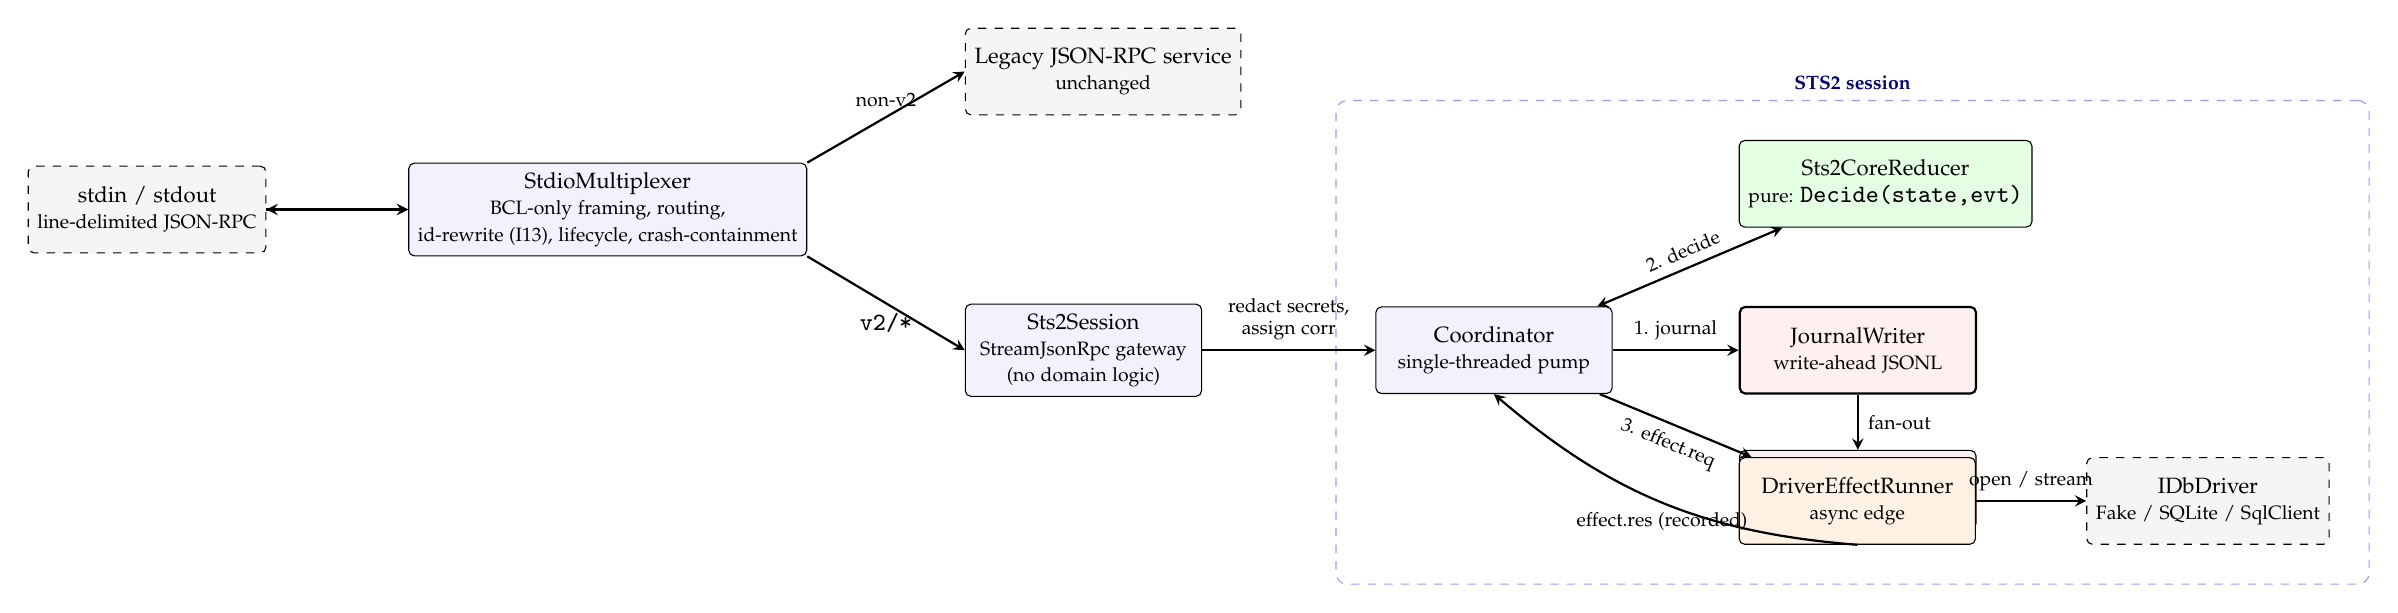
\begin{tikzpicture}[node distance=8mm and 14mm]
  \node[ext] (io) {stdin / stdout\\\scriptsize line-delimited JSON-RPC};
  \node[comp, right=18mm of io] (mux) {StdioMultiplexer\\\scriptsize BCL-only framing, routing,\\\scriptsize id-rewrite (I13), lifecycle, crash-containment};
  \node[ext, above right=6mm and 20mm of mux] (legacy) {Legacy JSON-RPC service\\\scriptsize unchanged};
  \node[comp, below right=6mm and 20mm of mux] (gw) {Sts2Session\\\scriptsize StreamJsonRpc gateway\\\scriptsize (no domain logic)};

  \draw[arr] (io) -- (mux);
  \draw[arr] (mux.north east) -- node[lbl,above]{non-v2} (legacy.west);
  \draw[arr] (mux.south east) -- node[lbl,below]{\code{v2/*}} (gw.west);
  \draw[arr,<->] (mux) -- (io);

  % STS2 internals
  \node[comp, right=22mm of gw] (coord) {Coordinator\\\scriptsize single-threaded pump};
  \draw[arr] (gw) -- node[lbl,above]{redact secrets,\\assign corr} (coord);

  \node[core, above right=10mm and 16mm of coord] (core) {Sts2CoreReducer\\\scriptsize pure: \code{Decide(state,evt)}};
  \node[jrnl, right=16mm of coord] (jr) {JournalWriter\\\scriptsize write-ahead JSONL};
  \node[sink, below=7mm of jr] (sinks) {aux sinks\\\scriptsize metrics, live tail, \dots};
  \node[edge, below right=8mm and 16mm of coord] (runner) {DriverEffectRunner\\\scriptsize async edge};
  \node[ext, right=14mm of runner] (drv) {IDbDriver\\\scriptsize Fake / SQLite / SqlClient};

  \draw[arr] (coord) -- node[lbl,above,sloped]{1. journal} (jr);
  \draw[arr] (jr) -- node[lbl,right]{fan-out} (sinks);
  \draw[arr,<->] (coord) -- node[lbl,above,sloped]{2. decide} (core);
  \draw[arr] (coord) -- node[lbl,below,sloped]{3. effect.req} (runner);
  \draw[arr] (runner) -- node[lbl,above]{open / stream} (drv);
  \draw[arr,bend left=18] (runner.south) to node[lbl,below]{effect.res (recorded)} (coord.south);

  \begin{scope}[on background layer]
    \node[draw=blue!40, dashed, rounded corners, fit=(coord)(core)(jr)(sinks)(runner)(drv), inner sep=5mm, label={[blue!50!black,font=\scriptsize\bfseries]above:STS2 session}] {};
  \end{scope}
\end{tikzpicture}}
\caption{STS2 runs inside the existing process, beside the legacy service, sharing one
stdio channel. The multiplexer routes \code{v2/*} to STS2 and everything else to legacy
untouched. Inside the session the gateway holds no domain logic; the Coordinator pump is the
only mover, and the Core reducer is the only decider.}
\end{figure}

%========================================================================================
\section*{2.\quad The event-capture seam: write-ahead journal $+$ best-effort fan-out}

\begin{figure}[H]
\centering
\resizebox{0.96\linewidth}{!}{%
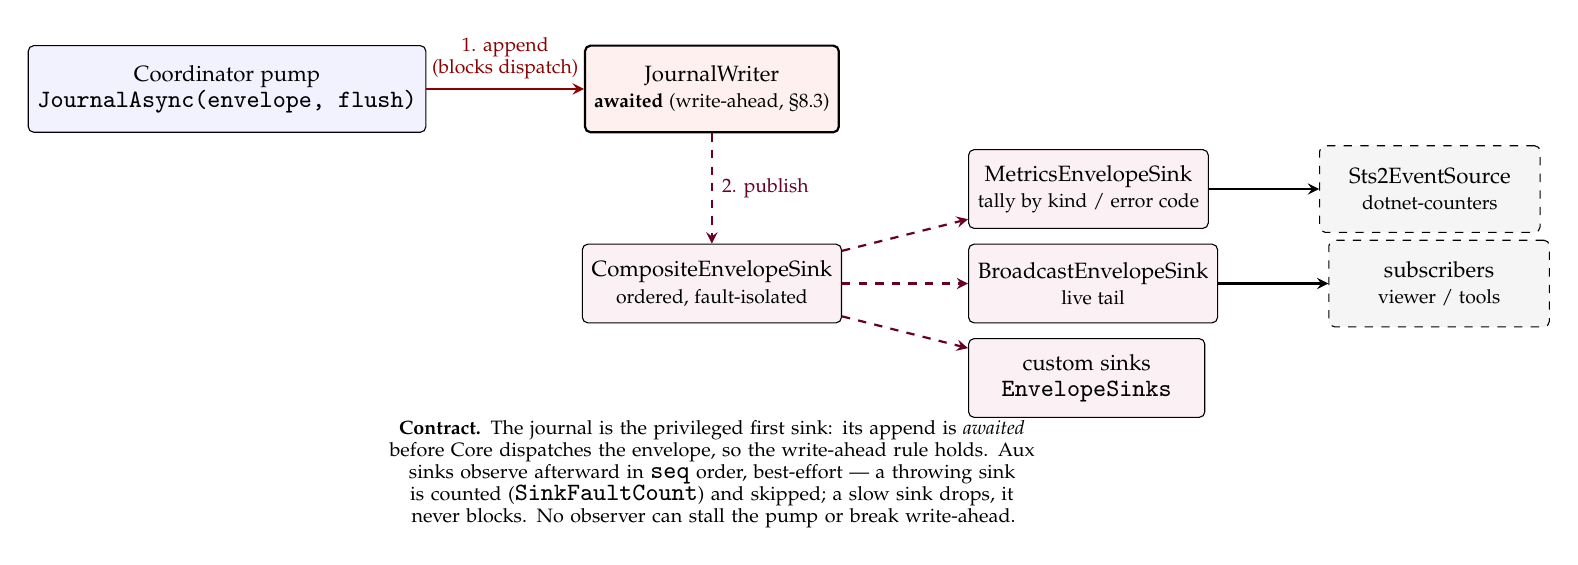
\begin{tikzpicture}[node distance=7mm and 16mm]
  \node[comp] (pump) {Coordinator pump\\\scriptsize \code{JournalAsync(envelope, flush)}};
  \node[jrnl, right=20mm of pump] (jr) {JournalWriter\\\scriptsize \textbf{awaited} (write-ahead, §8.3)};
  \node[sink, below=14mm of jr] (comp) {CompositeEnvelopeSink\\\scriptsize ordered, fault-isolated};

  \node[sink, right=16mm of comp, yshift=12mm] (met) {MetricsEnvelopeSink\\\scriptsize tally by kind / error code};
  \node[sink, right=16mm of comp] (bc) {BroadcastEnvelopeSink\\\scriptsize live tail};
  \node[sink, right=16mm of comp, yshift=-12mm] (cust) {custom sinks\\\scriptsize \code{EnvelopeSinks}};

  \node[ext, right=14mm of met] (es) {Sts2EventSource\\\scriptsize dotnet-counters};
  \node[ext, right=14mm of bc] (subs) {subscribers\\\scriptsize viewer / tools};

  \draw[warr] (pump) -- node[lbl,above]{1. append\\(blocks dispatch)} (jr);
  \draw[aarr] (jr) -- node[lbl,right]{2. publish} (comp);
  \draw[aarr] (comp) -- (met);
  \draw[aarr] (comp) -- (bc);
  \draw[aarr] (comp) -- (cust);
  \draw[arr] (met) -- (es);
  \draw[arr] (bc) -- (subs);

  \node[lbl, below=11mm of comp, text width=86mm] {%
    \textbf{Contract.} The journal is the privileged first sink: its append is \emph{awaited}
    before Core dispatches the envelope, so the write-ahead rule holds. Aux sinks observe
    afterward in \code{seq} order, best-effort --- a throwing sink is counted
    (\code{SinkFaultCount}) and skipped; a slow sink drops, it never blocks. No observer can
    stall the pump or break write-ahead.};
\end{tikzpicture}}
\caption{Observability is a fan-out seam (\code{IEnvelopeSink}), not a hard-wired consumer.
Solid red is the synchronous write-ahead path; dashed purple is the best-effort, fault-isolated
publish to auxiliary observers.}
\end{figure}

%========================================================================================
\section*{3.\quad Message lifecycle through the pump}

\begin{figure}[H]
\centering
\resizebox{0.99\linewidth}{!}{%
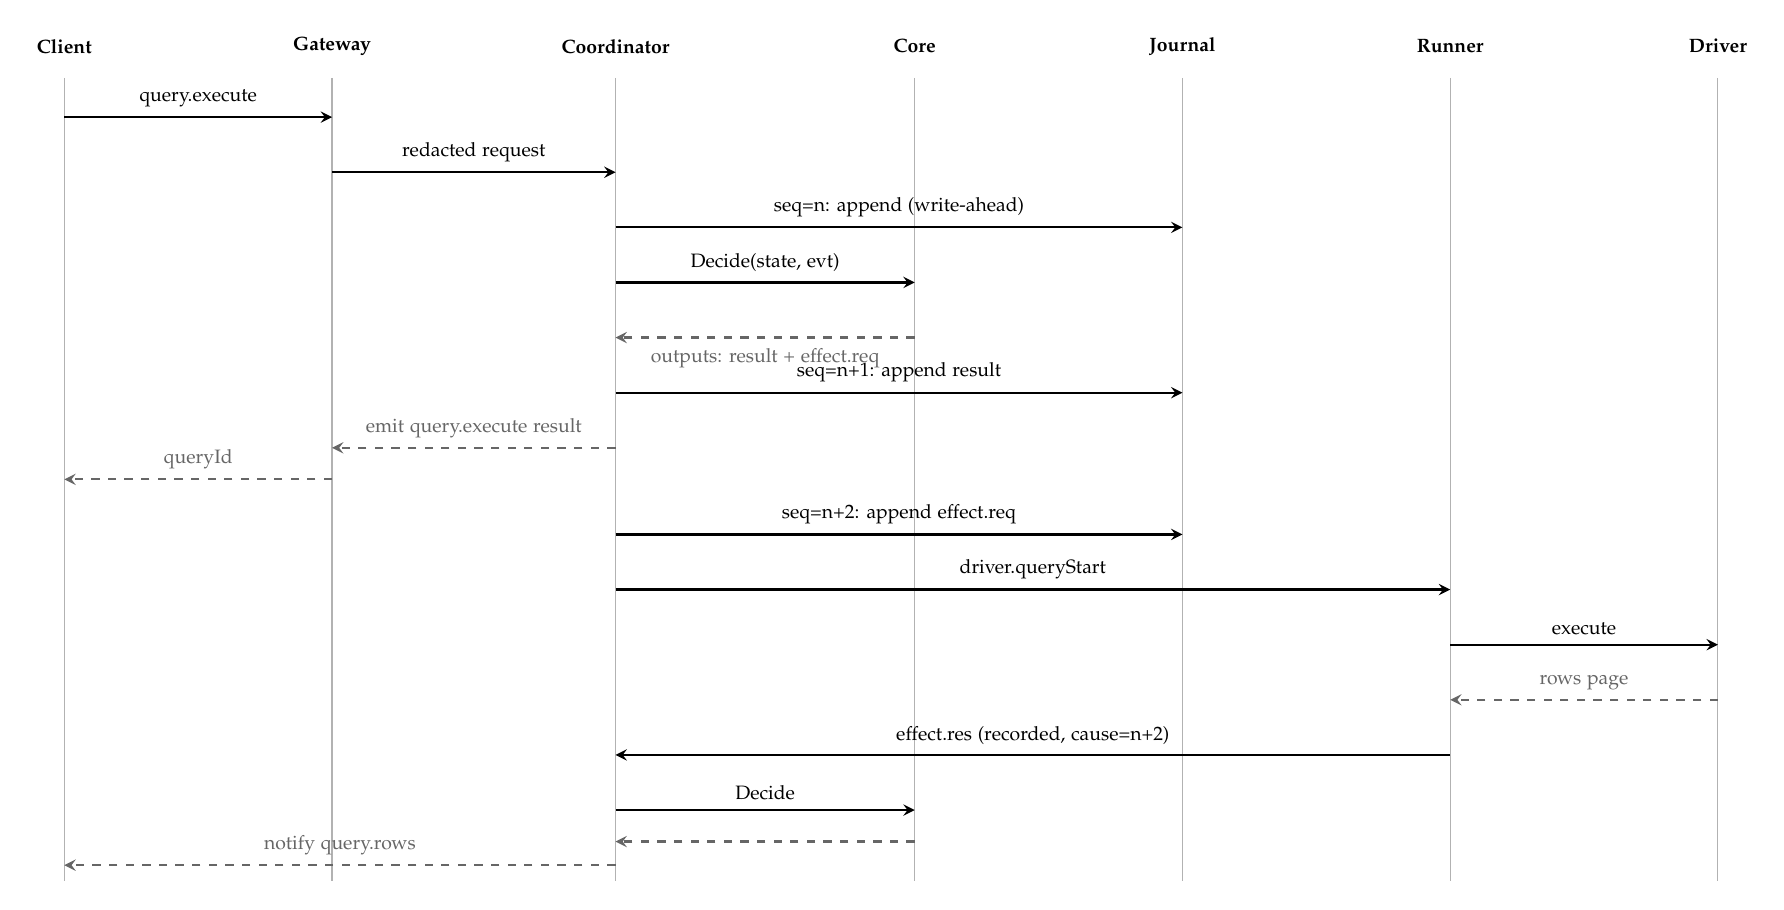
\begin{tikzpicture}[node distance=9mm]
  % lifelines
  \foreach \x/\name in {0/Client, 3.4/Gateway, 7.0/Coordinator, 10.8/Core, 14.2/Journal, 17.6/Runner, 21.0/Driver} {
    \node[font=\scriptsize\bfseries] (h\name) at (\x,0) {\name};
    \draw[black!30] (\x,-0.4) -- (\x,-10.6);
  }
  \tikzset{msg/.style={->, thick}, ret/.style={->, thick, dashed, black!60}}
  % sequence
  \draw[msg] (0,-0.9)   -- node[above,font=\scriptsize]{query.execute} (3.4,-0.9);
  \draw[msg] (3.4,-1.6) -- node[above,font=\scriptsize]{redacted request} (7.0,-1.6);
  \draw[msg] (7.0,-2.3) -- node[above,font=\scriptsize]{seq=n: append (write-ahead)} (14.2,-2.3);
  \draw[msg] (7.0,-3.0) -- node[above,font=\scriptsize]{Decide(state, evt)} (10.8,-3.0);
  \draw[ret] (10.8,-3.7) -- node[below,font=\scriptsize]{outputs: result + effect.req} (7.0,-3.7);
  \draw[msg] (7.0,-4.4) -- node[above,font=\scriptsize]{seq=n+1: append result} (14.2,-4.4);
  \draw[ret] (7.0,-5.1) -- node[above,font=\scriptsize]{emit query.execute result} (3.4,-5.1);
  \draw[ret] (3.4,-5.5) -- node[above,font=\scriptsize]{queryId} (0,-5.5);
  \draw[msg] (7.0,-6.2) -- node[above,font=\scriptsize]{seq=n+2: append effect.req} (14.2,-6.2);
  \draw[msg] (7.0,-6.9) -- node[above,font=\scriptsize]{driver.queryStart} (17.6,-6.9);
  \draw[msg] (17.6,-7.6) -- node[above,font=\scriptsize]{execute} (21.0,-7.6);
  \draw[ret] (21.0,-8.3) -- node[above,font=\scriptsize]{rows page} (17.6,-8.3);
  \draw[msg] (17.6,-9.0) -- node[above,font=\scriptsize]{effect.res (recorded, cause=n+2)} (7.0,-9.0);
  \draw[msg] (7.0,-9.7) -- node[above,font=\scriptsize]{Decide} (10.8,-9.7);
  \draw[ret] (10.8,-10.1) -- (7.0,-10.1);
  \draw[ret] (7.0,-10.4) -- node[above,font=\scriptsize]{notify query.rows} (0,-10.4);
\end{tikzpicture}}
\caption{One execute, end to end. Every external observation (the driver's rows page)
re-enters the pump as a \emph{recorded} \code{effect.res} envelope carrying a \code{cause}
pointer back to the effect request that produced it. Because nothing reaches Core except
journaled events, the journal alone is enough to replay the run.}
\end{figure}

%========================================================================================
\section*{4.\quad Journal-authoritative, wire-enriched: the overlay pattern}

\begin{figure}[H]
\centering
\resizebox{0.96\linewidth}{!}{%
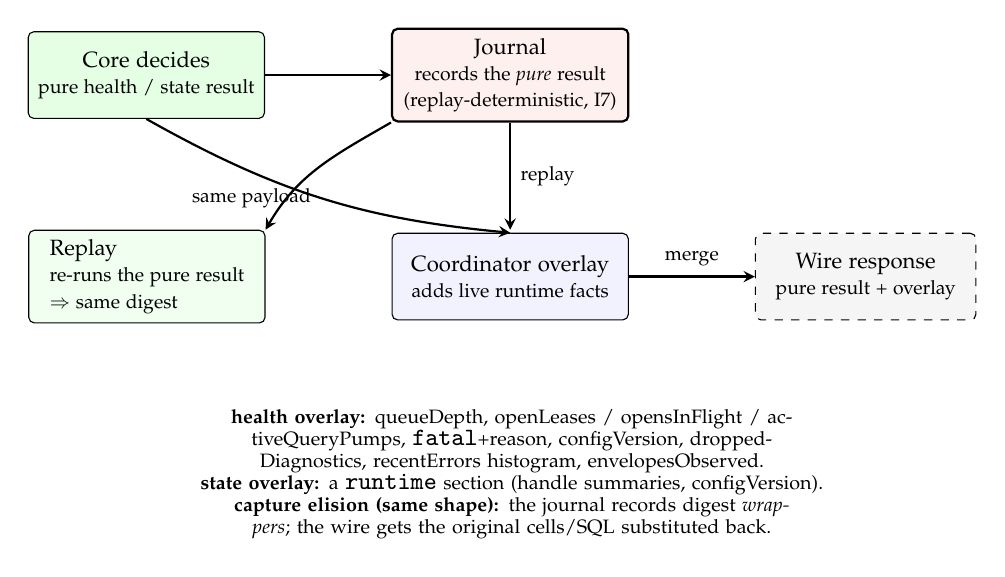
\begin{tikzpicture}[node distance=8mm and 16mm]
  \node[core] (dec) {Core decides\\\scriptsize pure health / state result};
  \node[jrnl, right=of dec] (jr) {Journal\\\scriptsize records the \emph{pure} result\\\scriptsize (replay-deterministic, I7)};
  \node[comp, below=14mm of jr] (ov) {Coordinator overlay\\\scriptsize adds live runtime facts};
  \node[ext, right=of ov] (wire) {Wire response\\\scriptsize pure result + overlay};
  \node[core, left=of ov, align=left, fill=green!6] (replay) {Replay\\\scriptsize re-runs the pure result\\\scriptsize $\Rightarrow$ same digest};

  \draw[arr] (dec) -- (jr);
  \draw[arr] (dec.south) to[bend right=12] node[lbl,left]{same payload} (ov.north);
  \draw[arr] (ov) -- node[lbl,above]{merge} (wire);
  \draw[arr] (jr) -- node[lbl,right]{replay} (replay.north-|jr) ;
  \draw[arr] (jr.south west) to[out=-150,in=60] (replay.north east);

  \node[lbl, below=10mm of ov, text width=100mm] {%
    \textbf{health overlay:} queueDepth, openLeases / opensInFlight / activeQueryPumps,
    \code{fatal}+reason, configVersion, droppedDiagnostics, recentErrors histogram, envelopesObserved.\\
    \textbf{state overlay:} a \code{runtime} section (handle summaries, configVersion).\\
    \textbf{capture elision (same shape):} the journal records digest \emph{wrappers}; the
    wire gets the original cells/SQL substituted back.};
\end{tikzpicture}}
\caption{Live introspection needs facts only the Runtime knows (queue depth, leases) ---
but those are non-deterministic, so journaling them would break replay. The fix, used by
health, state, and capture elision alike: the journal records the deterministic truth; the
coordinator overlays the live facts onto the wire response only. Replay sees the pure form
and stays digest-identical.}
\end{figure}

%========================================================================================
\section*{5.\quad Live tail: bounded, drop-oldest, counted}

\begin{figure}[H]
\centering
\resizebox{0.9\linewidth}{!}{%
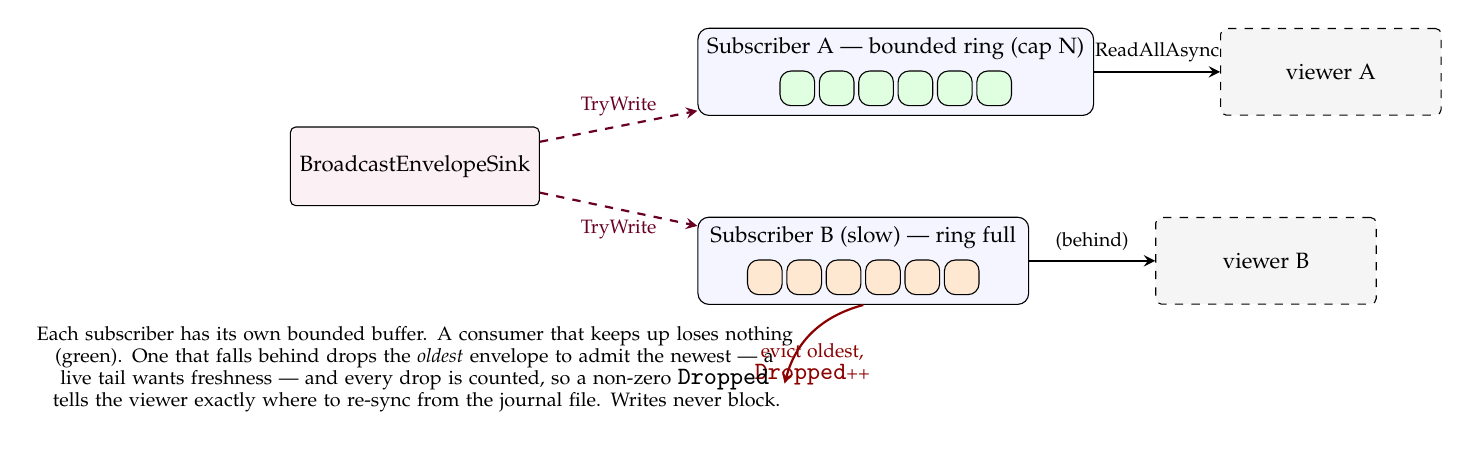
\begin{tikzpicture}[node distance=6mm and 16mm]
  \node[sink] (bc) {BroadcastEnvelopeSink};
  \node[draw, rounded corners, fill=blue!4, right=20mm of bc, yshift=12mm, minimum width=42mm, align=center] (s1)
    {Subscriber A — bounded ring (cap N)\\[1mm]
     \tikz{\foreach \i in {1,...,6}{\node[draw,minimum size=4.4mm,fill=green!12] at (\i*5mm,0){};}}};
  \node[draw, rounded corners, fill=blue!4, right=20mm of bc, yshift=-12mm, minimum width=42mm, align=center] (s2)
    {Subscriber B (slow) — ring full\\[1mm]
     \tikz{\foreach \i in {1,...,6}{\node[draw,minimum size=4.4mm,fill=orange!18] at (\i*5mm,0){};}}};
  \node[ext, right=16mm of s1] (cA) {viewer A};
  \node[ext, right=16mm of s2] (cB) {viewer B};

  \draw[aarr] (bc) -- node[lbl,above]{TryWrite} (s1);
  \draw[aarr] (bc) -- node[lbl,below]{TryWrite} (s2);
  \draw[arr] (s1) -- node[lbl,above]{ReadAllAsync} (cA);
  \draw[arr] (s2) -- node[lbl,above]{(behind)} (cB);
  \draw[warr] (s2.south) to[bend right=30] node[lbl,below]{evict oldest,\\ \code{Dropped}++} ($(s2.south)+(-1.0,-1.0)$);

  \node[lbl, below=14mm of bc, text width=96mm]{%
    Each subscriber has its own bounded buffer. A consumer that keeps up loses nothing
    (green). One that falls behind drops the \emph{oldest} envelope to admit the newest ---
    a live tail wants freshness --- and every drop is counted, so a non-zero \code{Dropped}
    tells the viewer exactly where to re-sync from the journal file. Writes never block.};
\end{tikzpicture}}
\caption{The diagnostic viewer's feed. Freshness over completeness, with an exact drop count
so gaps are detectable and recoverable.}
\end{figure}

%========================================================================================
\section*{6.\quad Runtime config change: \code{setCapture} $\to$ \code{config.changed} $\to$ replay-visible}

\begin{figure}[H]
\centering
\resizebox{0.98\linewidth}{!}{%
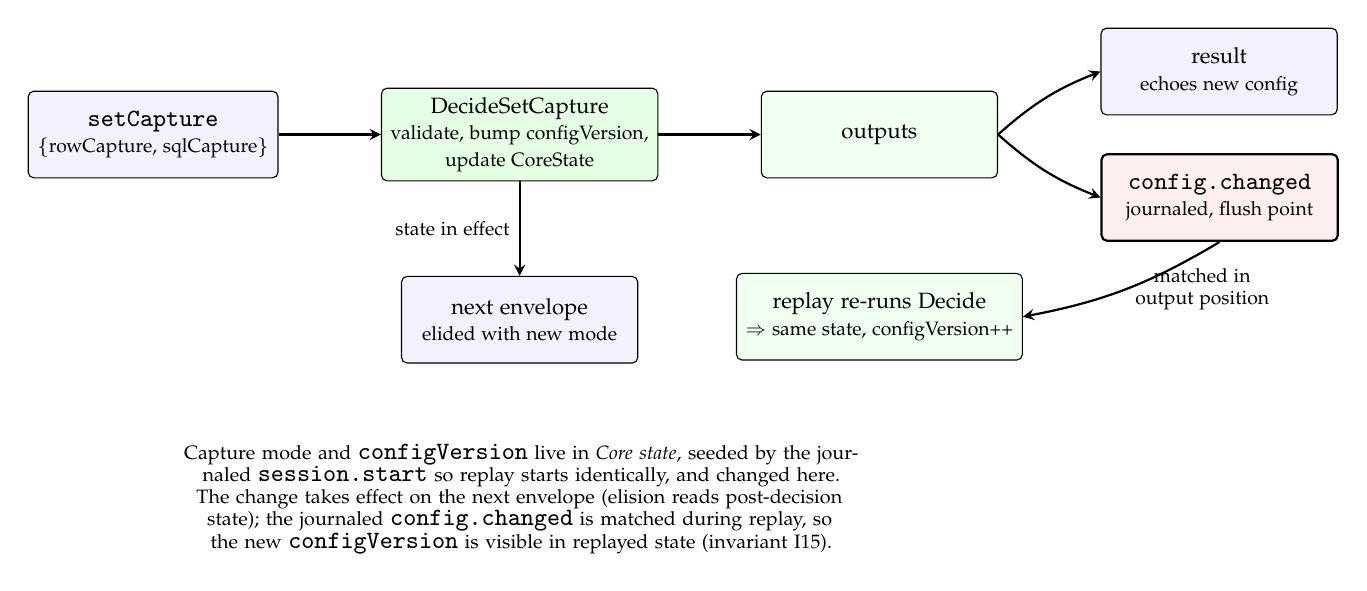
\begin{tikzpicture}[node distance=7mm and 13mm]
  \node[comp] (req) {\code{setCapture}\\\scriptsize \{rowCapture, sqlCapture\}};
  \node[core, right=of req] (dec) {DecideSetCapture\\\scriptsize validate, bump configVersion,\\\scriptsize update CoreState};
  \node[core, right=of dec, fill=green!6] (out) {outputs};
  \node[comp, right=of out, yshift=8mm] (res) {result\\\scriptsize echoes new config};
  \node[jrnl, right=of out, yshift=-8mm] (cc) {\code{config.changed}\\\scriptsize journaled, flush point};

  \draw[arr] (req) -- (dec);
  \draw[arr] (dec) -- (out);
  \draw[arr] (out.east) to[bend left=10] (res.west);
  \draw[arr] (out.east) to[bend right=10] (cc.west);

  \node[comp, below=12mm of dec, align=center] (next) {next envelope\\\scriptsize elided with new mode};
  \node[core, below=12mm of out, fill=green!6] (replay) {replay re-runs Decide\\\scriptsize $\Rightarrow$ same state, configVersion++};
  \draw[arr] (dec.south) -- node[lbl,left]{state in effect} (next.north);
  \draw[arr] (cc.south) to[bend left=10] node[lbl,right]{matched in\\output position} (replay.east);

  \node[lbl, below=9mm of next, text width=104mm]{%
    Capture mode and \code{configVersion} live in \emph{Core state}, seeded by the journaled
    \code{session.start} so replay starts identically, and changed here. The change takes
    effect on the next envelope (elision reads post-decision state); the journaled
    \code{config.changed} is matched during replay, so the new \code{configVersion} is visible
    in replayed state (invariant I15).};
\end{tikzpicture}}
\caption{Runtime reconfiguration is itself a journaled, replayable event --- not hidden
mutable state. The three formerly hard-coded \code{configVersion=1} literals are gone; the
version is sourced from Core state and stamped on every subsequent envelope.}
\end{figure}

%========================================================================================
\section*{7.\quad The Core state machines}

\begin{figure}[H]
\centering
\begin{minipage}{0.48\linewidth}\centering
\resizebox{\linewidth}{!}{%
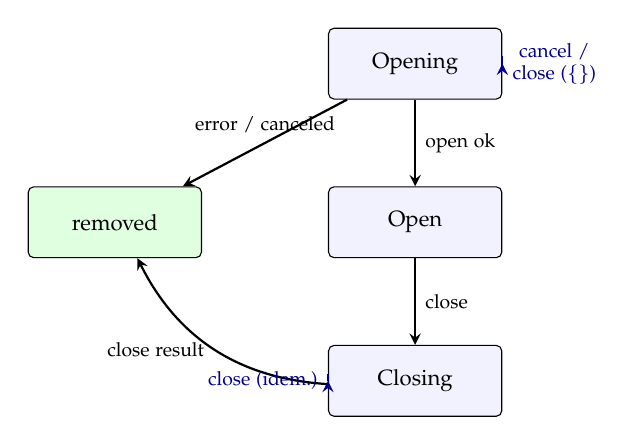
\begin{tikzpicture}[node distance=11mm]
  \node[st] (op) {Opening};
  \node[st, below=of op] (open) {Open};
  \node[st, below=of open] (cl) {Closing};
  \node[term, left=16mm of open] (gone) {removed};
  \draw[arr] (op) -- node[lbl,right]{open ok} (open);
  \draw[arr] (op) -- node[lbl,above]{error / canceled} (gone);
  \draw[arr] (open) -- node[lbl,right]{close} (cl);
  \draw[arr] (cl) to[bend left=30] node[lbl,left]{close result} (gone);
  \draw[larr] (op.east) to[out=20,in=-20,looseness=5] node[lbl,right]{cancel /\\ close (\{\})} (op.east);
  \draw[larr] (cl.west) to[out=160,in=-160,looseness=5] node[lbl,left]{close (idem.)} (cl.west);
\end{tikzpicture}}
\par\smallskip{\scriptsize\itshape Connection machine. One active query at a time; close cancels it first.}
\end{minipage}\hfill
\begin{minipage}{0.48\linewidth}\centering
\resizebox{\linewidth}{!}{%
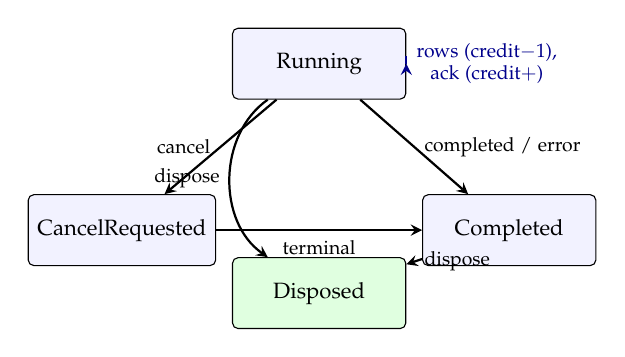
\begin{tikzpicture}[node distance=10mm]
  \node[st] (run) {Running};
  \node[st, below left=12mm and 2mm of run] (canc) {CancelRequested};
  \node[st, below right=12mm and 2mm of run] (comp) {Completed};
  \node[term, below=20mm of run] (disp) {Disposed};
  \draw[arr] (run) -- node[lbl,left]{cancel} (canc);
  \draw[arr] (run) -- node[lbl,right]{completed / error} (comp);
  \draw[arr] (canc) -- node[lbl,below]{terminal} (comp);
  \draw[arr] (comp) -- node[lbl,right]{dispose} (disp);
  \draw[arr] (run) to[bend right=55] node[lbl,left]{dispose} (disp);
  \draw[larr] (run.east) to[out=30,in=-30,looseness=5] node[lbl,right]{rows (credit$-$1),\\ ack (credit$+$)} (run.east);
\end{tikzpicture}}
\par\smallskip{\scriptsize\itshape Query machine. \code{query.complete} fires exactly once (I2); no output after it (I3); unacked pages $\le$ window (I9).}
\end{minipage}
\caption{The concurrency-sensitive logic lives entirely in the pure reducer, so both
machines are testable as a function and reproducible by replay. Idempotent self-loops
(blue) return \code{\{\}} for unknown or terminal ids.}
\end{figure}

\end{document}
